\documentclass[10pt]{article}

\usepackage[margin=0.75in]{geometry}
\usepackage{amsmath, amssymb}
\usepackage{graphicx}
\usepackage[T1]{fontenc}
\usepackage{inconsolata}
\usepackage{titlesec}
\usepackage{fancyhdr}
\usepackage{microtype}

\graphicspath{{../}}

\setlength{\parindent}{0pt}
\setlength{\parskip}{2pt}
\renewcommand{\baselinestretch}{1.0}

\titleformat{\section}{\ttfamily\normalsize\bfseries\MakeUppercase}{\thesection}{0.6em}{}
\titlespacing*{\section}{0pt}{8pt}{2pt}
\titleformat{\subsection}{\ttfamily\small\MakeUppercase}{\thesubsection}{0.6em}{}
\titlespacing*{\subsection}{0pt}{6pt}{2pt}

\pagestyle{fancy}
\fancyhf{}
\renewcommand{\headrulewidth}{0pt}
\renewcommand{\footrulewidth}{0.5pt}
\fancyfoot[L]{\ttfamily\footnotesize PARAPET-WIND-CC}
\fancyfoot[C]{\ttfamily\footnotesize REV \today}
\fancyfoot[R]{\ttfamily\footnotesize \thepage}

\begin{document}

\noindent
\includegraphics[height=0.7cm]{logo}\hfill
{\ttfamily\normalsize\bfseries\MakeUppercase{Parapet Lateral Load --- Components and Cladding}}\quad
{\ttfamily\footnotesize\today}
\vspace{4pt}\hrule\vspace{6pt}


\section{Method Selection}

{\ttfamily\footnotesize\bfseries DECISION}

{\ttfamily\footnotesize
\begin{tabular}{@{}ll@{}}
$h = 25$ ft $\le 60$ ft & Part 4 (Eq.\ 30.6-1) does NOT apply \\
--- & Part 4 scope is 60 ft $< h \le 160$ ft \\
governing & Part 6, \S30.8, Eq.\ (30.8-1) \\
note & \S30.9 is roof overhangs, not parapets \\
\end{tabular}}

\medskip{\ttfamily\footnotesize\bfseries ASSUMPTIONS}

{\ttfamily\footnotesize
\begin{tabular}{@{}ll@{}}
roof & flat, $\theta \le 7^\circ$ (Fig.\ 30.3-2A) \\
enclosure & enclosed building \\
parapet & solid knee wall; no envelope $\Rightarrow (GC_{pi}) = 0$ \\
$K_{zt}$, $K_e$ & 1.0 \\
\end{tabular}}

\section{Inputs}

{\ttfamily\footnotesize
\begin{tabular}{@{}ll@{}}
$V$ & 153 mph \\
exposure & D \\
$h$ & 25 ft \\
$h_p$ & 3 ft \\
$h + h_p$ & 28 ft (top of parapet) \\
studs & 2$\times$6 knee studs at 16 in.\ o.c. \\
span & 3.29 ft (3'-3.5" cantilever above deck) \\
$A$ & 4.4 ft$^2$ $=$ 3.29 $\times$ 1.33 \\
\end{tabular}}

\section{Velocity Pressure}

\begin{equation}
q_p = 0.00256\,K_z K_{zt} K_d K_e V^2 \tag{ASCE 7-16 Eq.\ 26.10-1}
\end{equation}

{\ttfamily\footnotesize
\begin{tabular}{@{}ll@{}}
$q_p$ & velocity pressure at top of parapet, psf \\
$K_z$ & 1.144 at $z=28$ ft, Exp.\ D (Table 26.10-1, interp.\ 25--30 ft) \\
$K_d$ & 0.85, C\&C (Table 26.6-1) \\
$K_e$ & 1.00 (Table 26.9-1) \\
\end{tabular}}

\begin{equation*}
q_p = 0.00256(1.144)(1.0)(0.85)(1.0)(153)^2 = 58.3\ \text{psf}
\end{equation*}

\section{External Pressure Coefficients}

\noindent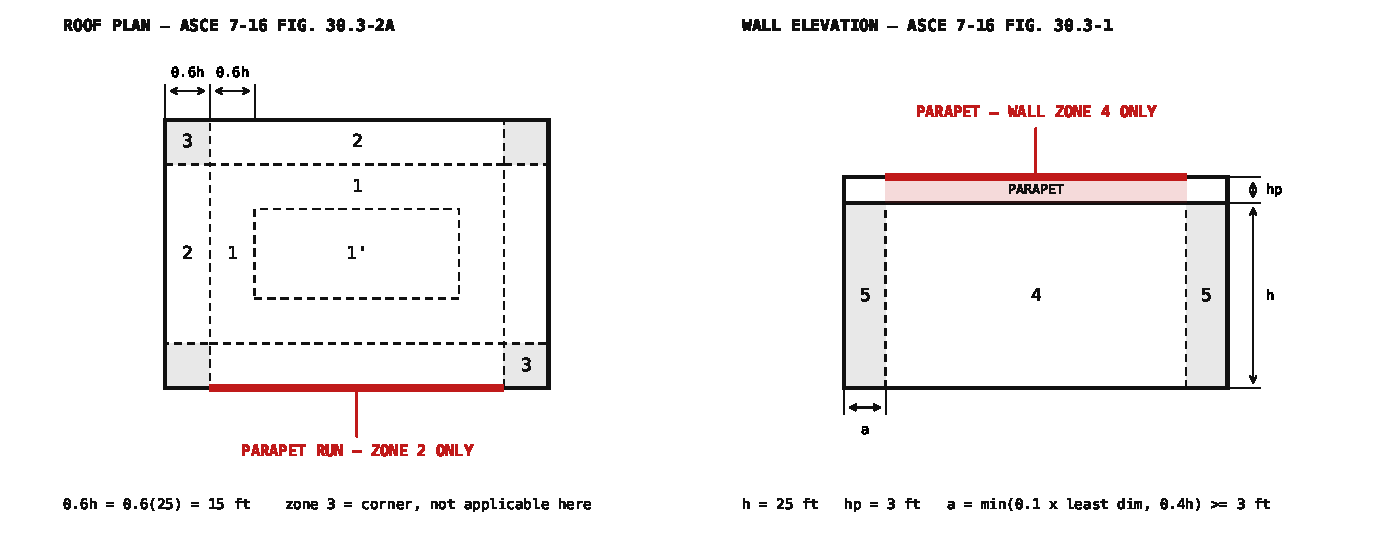
\includegraphics[width=\textwidth]{zones}

\medskip

{\ttfamily\footnotesize WHERE: Figs.\ 30.3-1, 30.3-2A. $A = 4.4$ ft$^2 \le 10$ ft$^2$: plateau values, no interpolation.}

{\ttfamily\footnotesize
\begin{tabular}{@{}lll@{}}
SURFACE & ZONE & $(GC_p)$ \\
wall, positive (Fig.\ 30.3-1) & 4 & $+1.00$ \\
wall, negative (Fig.\ 30.3-1) & 4 & $-1.10$ \\
roof, negative (Fig.\ 30.3-2A) & 2 & $-2.30$ \\
\end{tabular}}

\medskip{\ttfamily\footnotesize\bfseries EFFECTIVE WIND AREA}

{\ttfamily\footnotesize
\begin{tabular}{@{}ll@{}}
element & 2$\times$6 knee stud, vertical cantilever \\
$A$ & span $\times$ trib $=$ 3.29 $\times$ 1.33 $=$ 4.4 ft$^2$ \\
\S26.2 & width 1.33 ft $\ge$ span$/3 = 1.10$ ft \\
--- & $A \le 10$ ft$^2$ $\Rightarrow$ flat of curve, most severe $(GC_p)$ \\
\end{tabular}}

\medskip
\noindent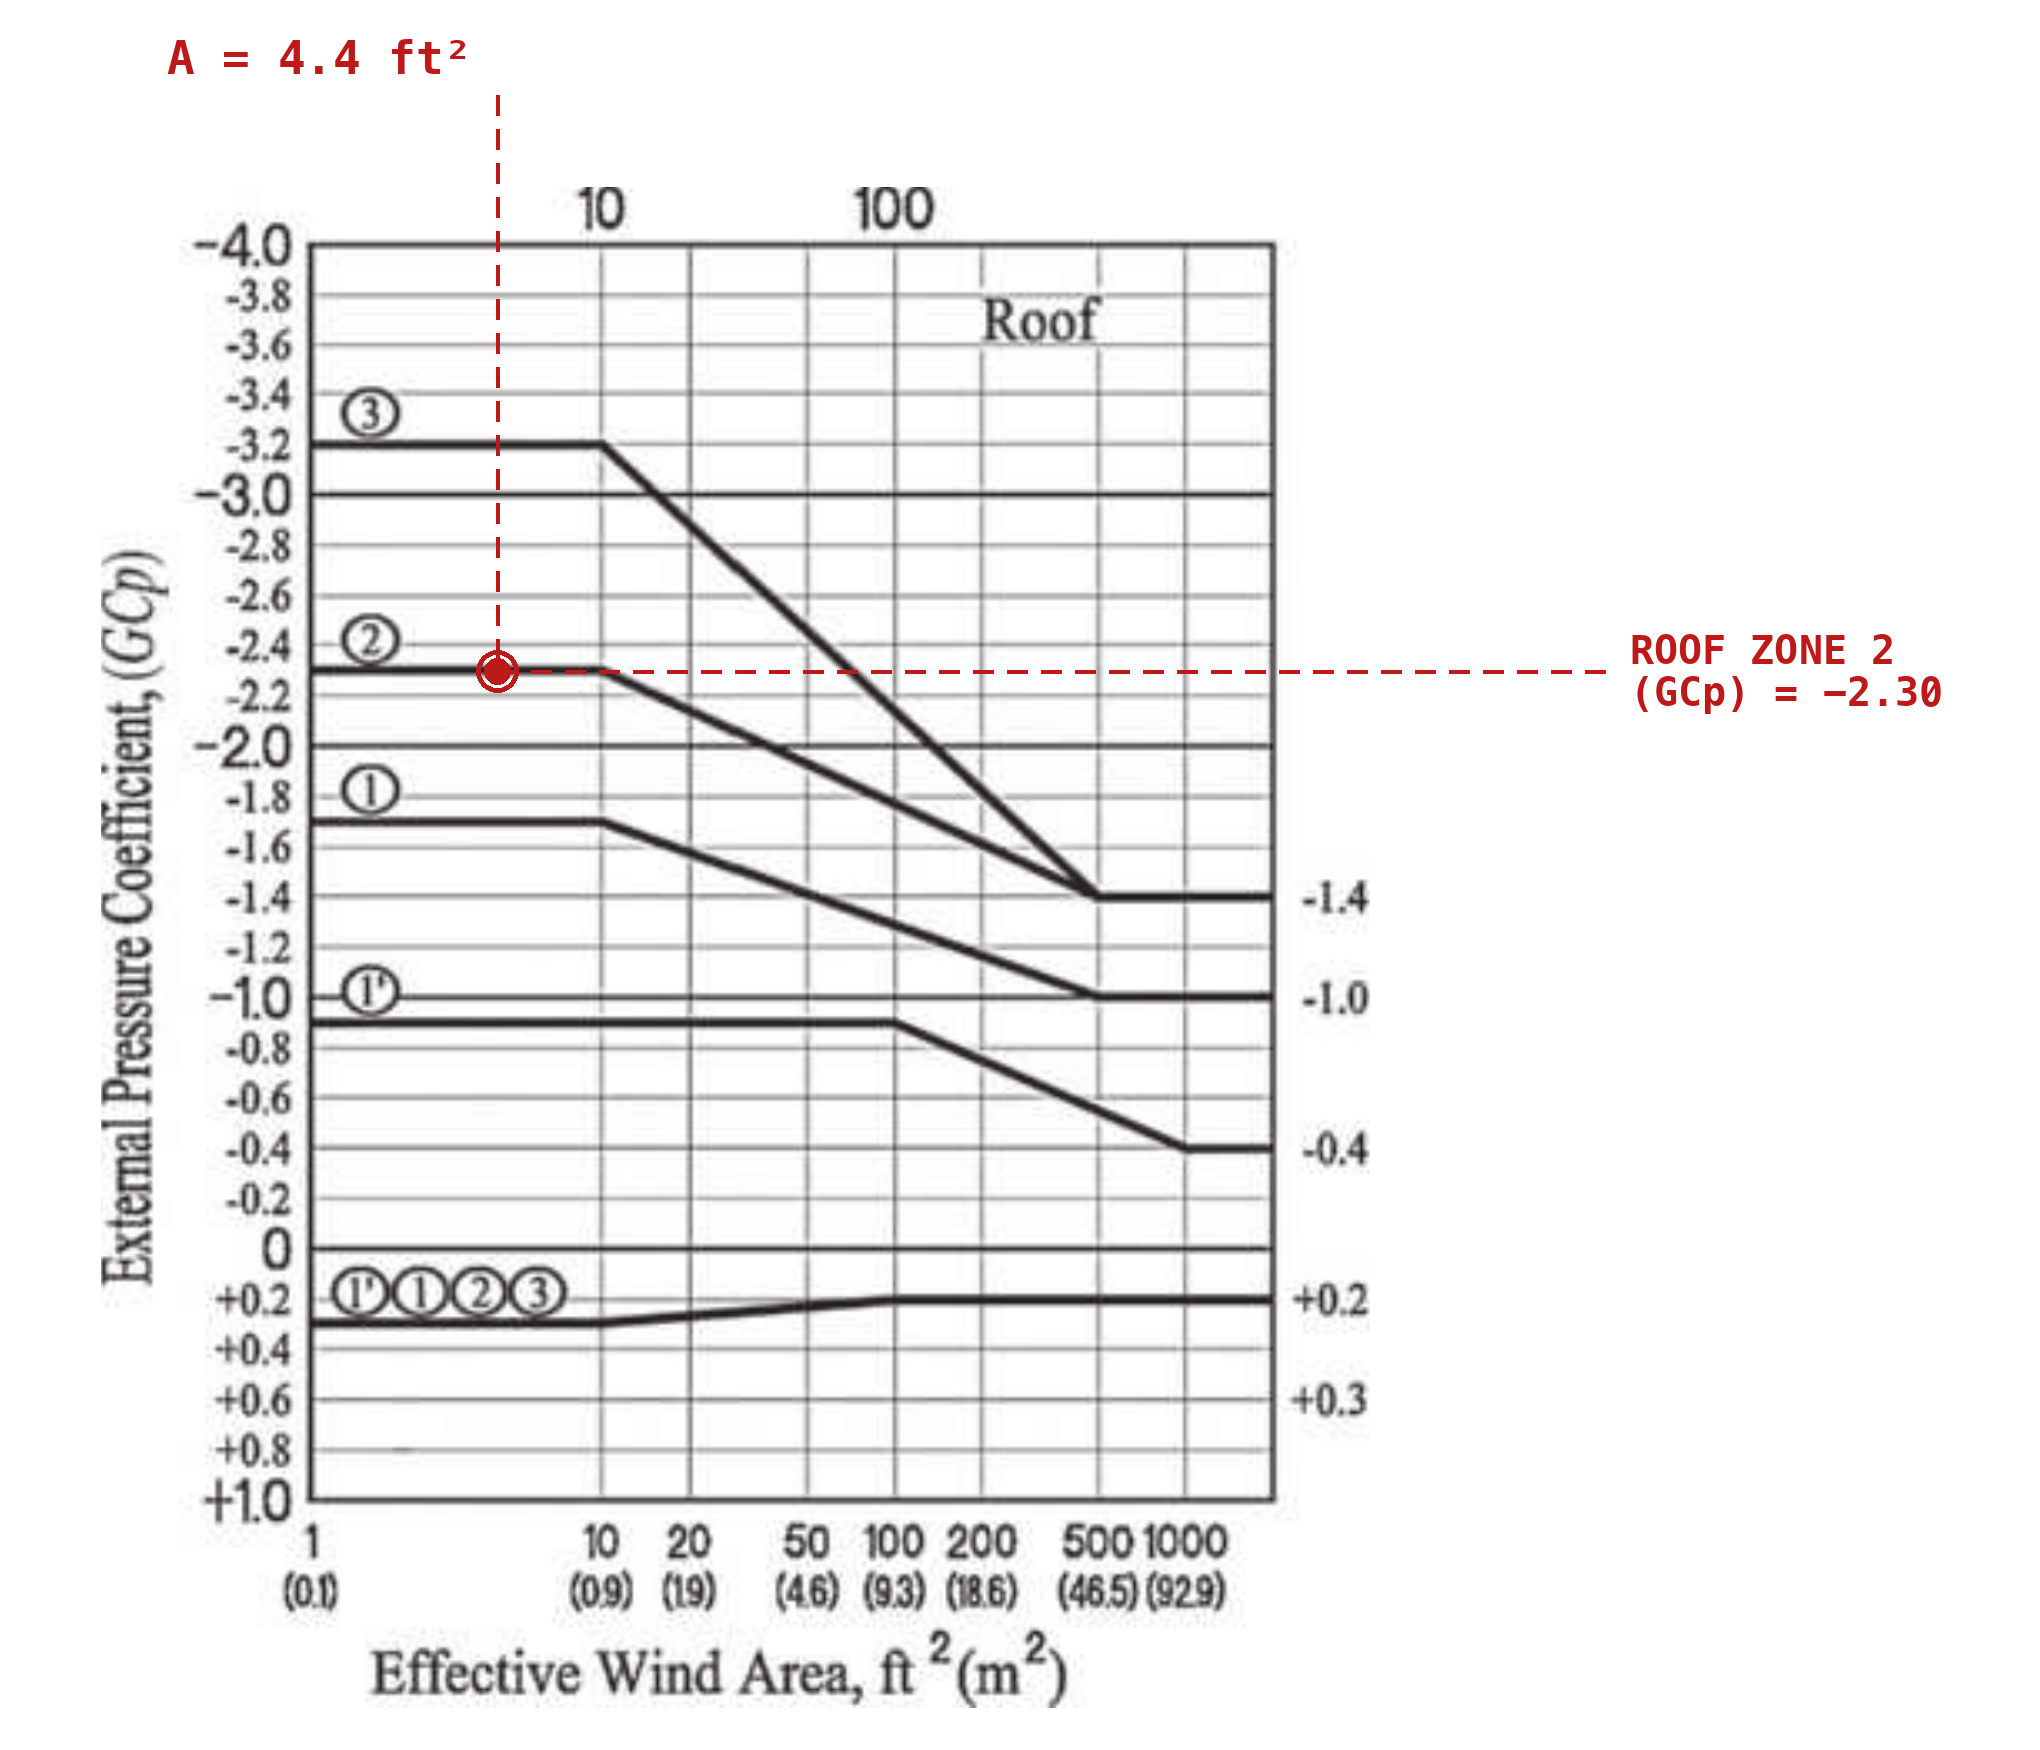
\includegraphics[width=0.385\textwidth]{gcp-roof}\hfill
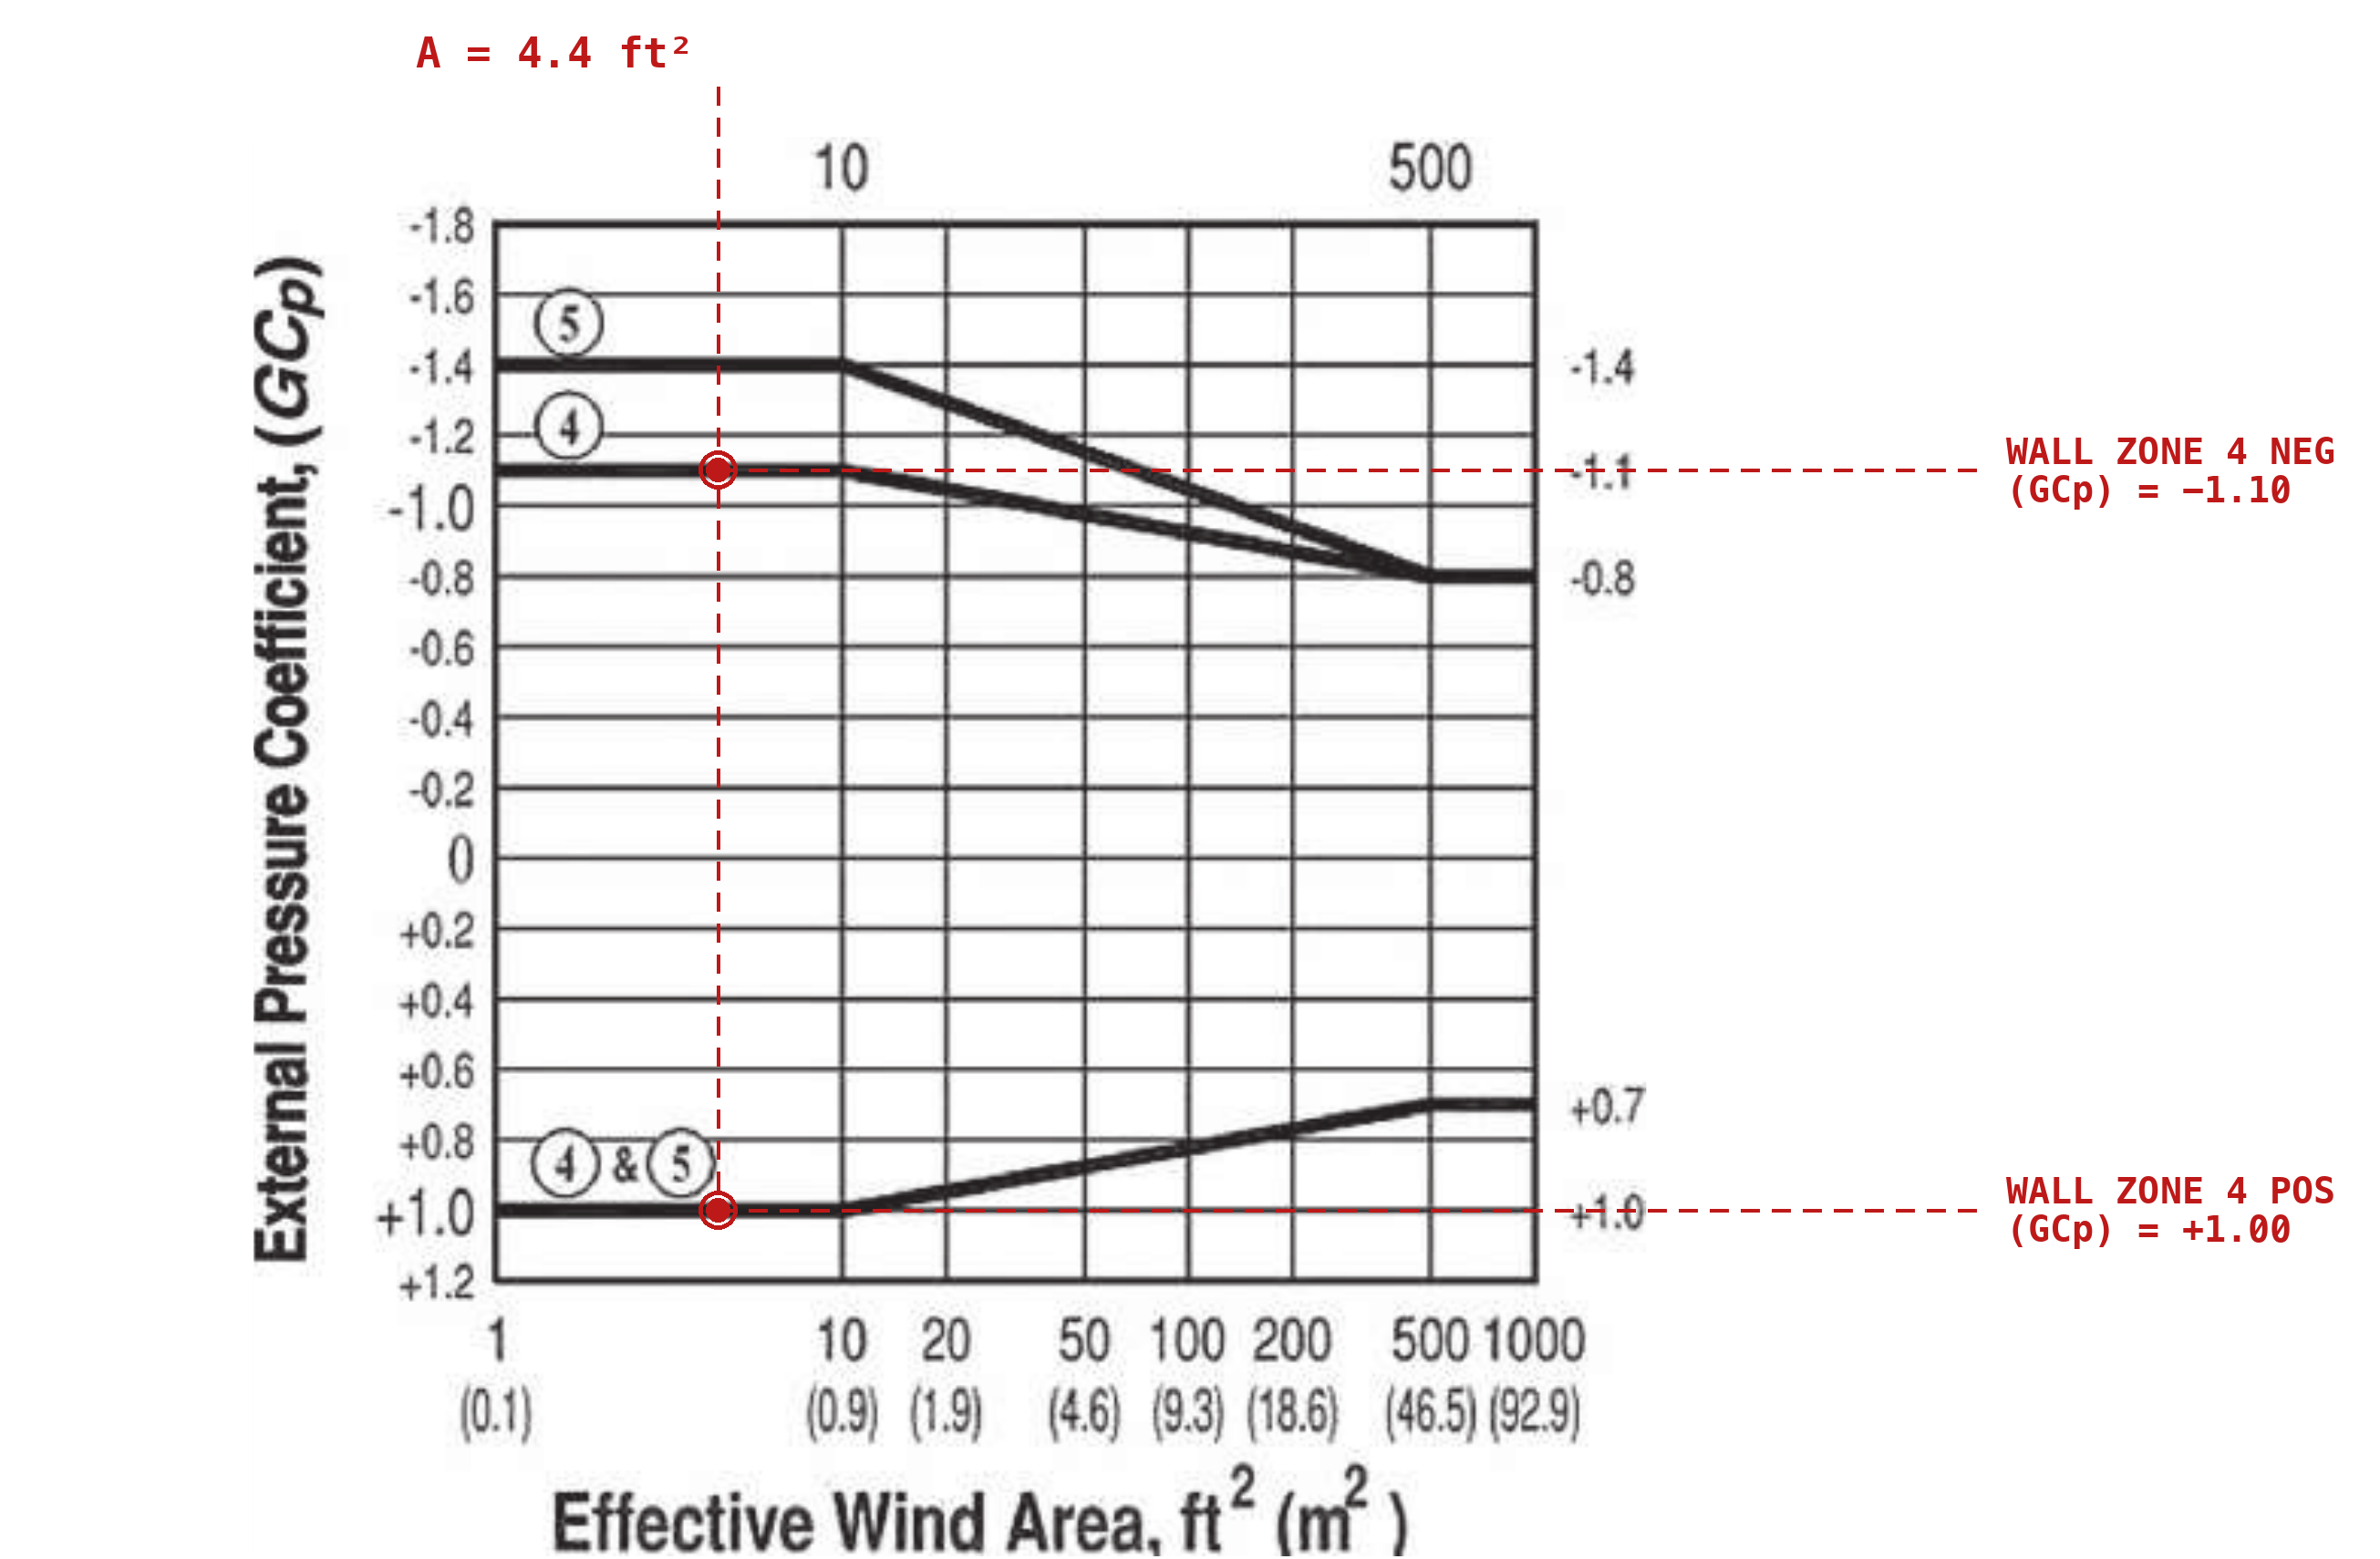
\includegraphics[width=0.435\textwidth]{gcp-wall}

{\ttfamily\scriptsize ASCE 7-16 Fig.\ 30.3-2A (roof, $\theta \le 7^\circ$) and Fig.\ 30.3-1 (walls); read at $A = 4.4$ ft$^2$.}

\medskip{\ttfamily\footnotesize\bfseries LIMITS}

{\ttfamily\footnotesize
\begin{tabular}{@{}ll@{}}
zone scope & parapet run is interior edge only; no corner \\
--- & Zone 3 (roof) and Zone 5 (wall) do not apply \\
Fig.\ 30.3-1 Note 5 & wall $(GC_p)$ may be cut 10\% when $\theta \le 10^\circ$; not taken \\
\end{tabular}}

\section{Design Pressure}

\begin{equation}
p = q_p\left[(GC_p) - (GC_{pi})\right] \tag{ASCE 7-16 Eq.\ 30.8-1}
\end{equation}

{\ttfamily\footnotesize
\begin{tabular}{@{}ll@{}}
WHERE & Fig.\ 30.8-1, two load cases per \S30.8 \\
$(GC_{pi})$ & per porosity of the parapet envelope; $=0$ here \\
Case A & windward parapet: $+$wall front, $-$roof Zone 2 back \\
Case B & leeward parapet: $+$wall back, $-$wall Zone 4 front \\
\end{tabular}}

\medskip
\noindent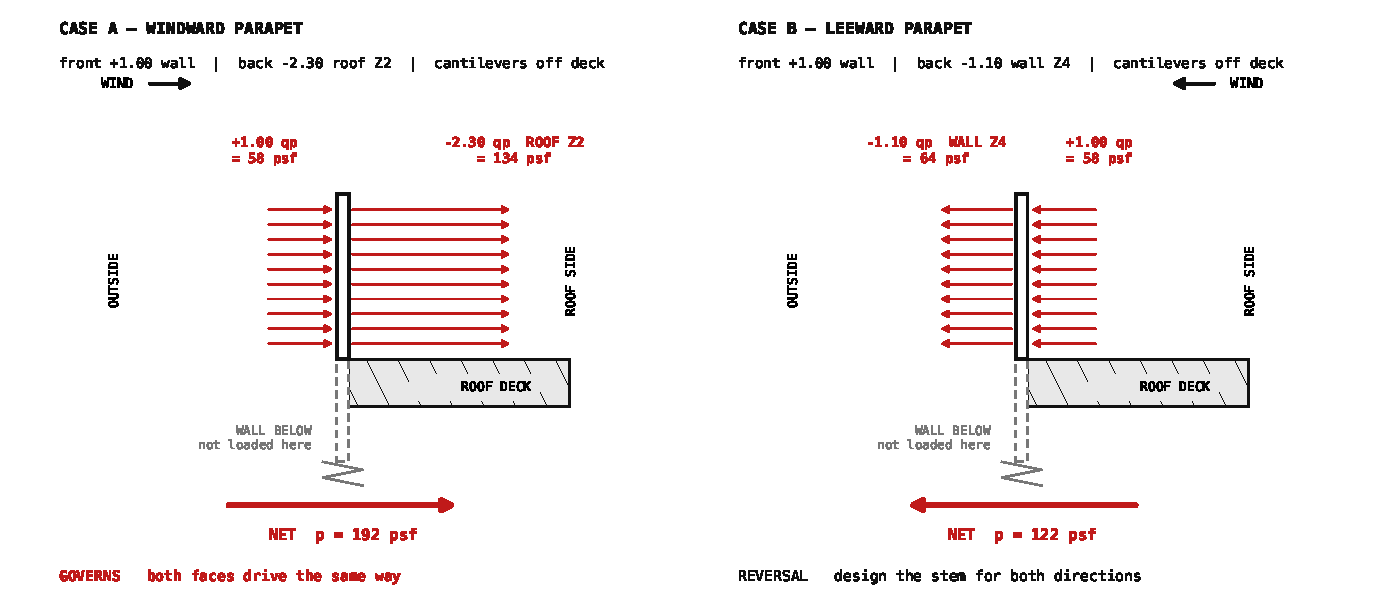
\includegraphics[width=0.90\textwidth]{cases}

\medskip
{\ttfamily\footnotesize
\begin{tabular}{@{}llrr@{}}
CASE & SURFACES & NET $(GC_p)$ & $p$ (psf) \\
A & wall $+1.00$ / roof Z2 $-2.30$ & 3.30 & 192 \\
B & wall $+1.00$ / wall Z4 $-1.10$ & 2.10 & 122 \\
\end{tabular}}

\section{Governing}

{\ttfamily\footnotesize
\begin{tabular}{@{}ll@{}}
Case A & $p = 192$ psf (windward parapet, roof Zone 2) \\
direction & acts horizontally, normal to parapet face \\
\end{tabular}}

\end{document}
